% Этот шаблон документа разработан в 2014 году
% Данилом Фёдоровых (danil@fedorovykh.ru) 
% для использования в курсе 
% <<Документы и презентации в \LaTeX>>, записанном НИУ ВШЭ
% для Coursera.org: http://coursera.org/course/latex .
% Исходная версия шаблона --- 
% https://www.writelatex.com/coursera/latex/5.1

\documentclass[t]{beamer}  % [t], [c], или [b] --- вертикальное выравнивание на слайдах (верх, центр, низ)
%\documentclass[handout]{beamer} % Раздаточный материал (на слайдах всё сразу)
%\documentclass[aspectratio=169]{beamer} % Соотношение сторон

%\usetheme{default}
%\usetheme{AnnArbor}
%\usetheme{Antibes}
%\usetheme{Bergen}
%\usetheme{Berkeley}
%\usetheme{Berlin}
%\usetheme{Boadilla}
%\usetheme{CambridgeUS}
%\usetheme{Copenhagen}
%\usetheme{Darmstadt}
%\usetheme{Dresden}
%\usetheme{Frankfurt}
%\usetheme{Goettingen}
%\usetheme{Hannover}
%\usetheme{Ilmenau}
%\usetheme{JuanLesPins}
%\usetheme{Luebeck}
\usetheme{Madrid}
%\usetheme{Malmoe}
%\usetheme{Marburg}
%\usetheme{Montpellier}
%\usetheme{PaloAlto}
%\usetheme{Pittsburgh}
%\usetheme{Rochester}
%\usetheme{Singapore}
%\usetheme{Szeged}
%\usetheme{Warsaw}

%\usecolortheme{beaver} % Цветовая схема
%\useinnertheme{circles}
%\useinnertheme{rectangles}


%%% Работа с русским языком

\usepackage{cmap}					% поиск в PDF
\usepackage{mathtext} 				% русские буквы в формулах
\usepackage[T2A]{fontenc}			% кодировка
\usepackage[utf8]{inputenc}			% кодировка исходного текста
\usepackage[english,russian]{babel}	% локализация и переносы

%% Beamer по-русски
\newtheorem{rtheorem}{Теорема}
\newtheorem{rproof}{Доказательство}
\newtheorem{rexample}{Пример}

%%% Дополнительная работа с математикой
\usepackage{amsmath,amsfonts,amssymb,amsthm,mathtools} % AMS
\usepackage{icomma} % "Умная" запятая: $0,2$ --- число, $0, 2$ --- перечисление

\pagestyle{plain}
\beamertemplatenavigationsymbolsempty
%% Номера формул
%\mathtoolsset{showonlyrefs=true} % Показывать номера только у тех формул, на которые есть \eqref{} в тексте.
%\usepackage{leqno} % Нумерация формул слева

%% Свои команды
\DeclareMathOperator{\sgn}{\mathop{sgn}}

%% Перенос знаков в формулах (по Львовскому)
\newcommand*{\hm}[1]{#1\nobreak\discretionary{}
{\hbox{$\mathsurround=0pt #1$}}{}}

%%% Работа с картинками
\usepackage{graphicx}  % Для вставки рисунков
\graphicspath{{img/}{images2/}}  % папки с картинками
\setlength\fboxsep{3pt} % Отступ рамки \fbox{} от рисунка
\setlength\fboxrule{1pt} % Толщина линий рамки \fbox{}
\usepackage{wrapfig} % Обтекание рисунков текстом

%%% Работа с таблицами
\usepackage{array,tabularx,tabulary,booktabs} % Дополнительная работа с таблицами
\usepackage{longtable}  % Длинные таблицы
\usepackage{multirow} % Слияние строк в таблице

%%% Программирование
\usepackage{etoolbox} % логические операторы

%%% Другие пакеты
\usepackage{lastpage} % Узнать, сколько всего страниц в документе.
\usepackage{soul} % Модификаторы начертания
\usepackage{csquotes} % Еще инструменты для ссылок
%\usepackage[style=authoryear,maxcitenames=2,backend=biber,sorting=nty]{biblatex}
\usepackage{multicol} % Несколько колонок

%%% Картинки
\usepackage{tikz} % Работа с графикой
\usepackage{pgfplots}
\usepackage{pgfplotstable}
\usepackage{listings}





\title{Использование статического анализа \\ корректно-синхронизированного кода \\ для ускорения динамического поиска конфликтов}
\subtitle{}
\author{Выполнил: Роскошный Яков Игоревич \\ Руководитель: Цителов Дмитрий Игоревич}
\institute{Университет ИТМО}

\begin{document}

\frame[plain]{\titlepage}	% Титульный слайд

\section{Проблема и задача}
\begin{frame}[fragile]
  \frametitle{Решаемая проблема}

\begin{figure}[h]
\center
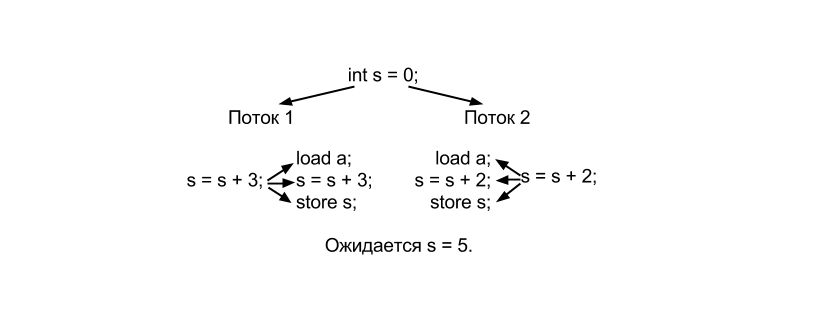
\includegraphics[width=10cm,height=4cm]{RaceCondition.png}
\end{figure}

\begin{itemize}
    \item При отсутствии синхронизации между двумя потоками может возникнуть гонка.
    \item В итоге результат работы программы будет недетерминирован.
  \end{itemize}
\end{frame}
\begin{frame}[fragile]
  \frametitle{Решаемая проблема}
\begin{itemize}
    \item Состояние гонки (data race, race condition) - несинхронизированные обращения из различных потоков к одному и тому же участку памяти, хотя бы одно из которых является обращением на запись
    \item Состояние гонки в программах является частой допускаемой ошибкой, и обнаружение данных ошибок является сложной и актуальной задачей.
    \item Cуществует два принципиально разных подхода к обнаружению гонок: статический и динамический.
  \end{itemize}
\end{frame}
\begin{frame}[fragile]
  \frametitle{Решаемая проблема}
\begin{itemize}
    \item Задача нахождения гонок статическим анализом является NP-трудной. 
    \item Существующие утилиты статического анализа используют различные эвристики, уменьшают глубину анализа, что приводит к существенно неточным и неполным результатам, а также допускают ложные срабатывания
    \item Динамические детекторы выполняются одновременно с программой и отслеживают синхронизационные события и обращения к разделяемым переменным.
    \item Главной проблемой динамического подхода является наносимый ущерб производительности и потребления памяти
анализируемой программы.
  \end{itemize}
\end{frame}


\begin{frame}[fragile]
  \frametitle{Постановка задачи}
\begin{itemize}
    \item Большинство динамических детекторов хранит структуры данных для полей.
    \item Статическим анализом можно выяснить, что некоторые поля корректо-синхронизированы. Аналогично, можно доказать, что метод корректно-синхронизирован. 
    \item Корректно-синхронизированный код можно исключить из динамического анализа.
    \item Это позволит уменьшить потребление памяти и времени динамических детекторов.
  \end{itemize}
\end{frame}

\begin{frame}[fragile]
  \frametitle{Цели работы}
  \vspace{0.5cm}  
\begin{itemize}
	\setlength\itemsep{1cm}
	\item Разработка алгоритма и утилиты для статического поиска корректно-синхронизированного кода на Java.
	\item Интеграция утилиты с динамическим детектором jDRD - детектор гонок для Java программ.
    	\item Ускорение jDRD. 

    \end{itemize}
\end{frame}



\begin{frame}[fragile]
  \frametitle{Алгоритм решения задачи}
  \vspace{0.5cm}  
\begin{itemize}
    \setlength\itemsep{1cm}
    \item Востановить граф потока управления (control flow graph) для каждого метода.

    \item Провести анализ того, какие переменные могут быть блокировкой. 

    \item Для каждого метода обойти его CFG, анализируя множество взятых блокировок и операции чтения/записи полей.
  \end{itemize}
\end{frame}

\begin{frame}[fragile]
  \frametitle{Алгоритм решения задачи. Промежуточные представление}
  \vspace{0.5cm}  
\begin{itemize}
    \setlength\itemsep{1cm}
    \item Строить CFG основываясь на байт-код представлении или на исходных файлах программы не всегда удобно.
    \item Байт-код содержит большое количество операций, а исходный код java многочисленные синтаксические конструкции.
    \item Поэтому оказывается удобным использовать промежуточные представления. 
  \end{itemize}
\end{frame}

\begin{frame}[fragile]
  \frametitle{Алгоритм решения задачи. Промежуточные представление}
  \begin{itemize}
    \item В данной работе проводился анализ основываясь на SSA(Single state assignment) представлении промежуточного кода.  Данный код строится на основе байт-кода, но обладает отличительными особенностями:
	 \begin{itemize}
	    \setlength\itemsep{0.5cm}
            \item Стек полностью заменен на локальные переменные.
	    \item Операции сгруппированы. Различных типов операций около 20.
	    \item Каждая локальная переменная имеет единственное присваивание.
	 \end{itemize} 
  \end{itemize}
\end{frame}

\begin{frame}[fragile]
  \frametitle{Алгоритм решения задачи. Control flow graph}


  \begin{columns}
 		\column{0.3\textwidth}
			\vspace{2cm}
			\begin{lstlisting}[basicstyle=\tiny, language=Java]
			public class A {
			  int x = 0;
			  public void a() {
			    while (x % 2 == 0) {
			      x++;
			    }
			  }
			}
			 \end{lstlisting}
                 \column{0.65\textwidth}
			  \begin{figure}[h]
				  \vspace{0pt}
				  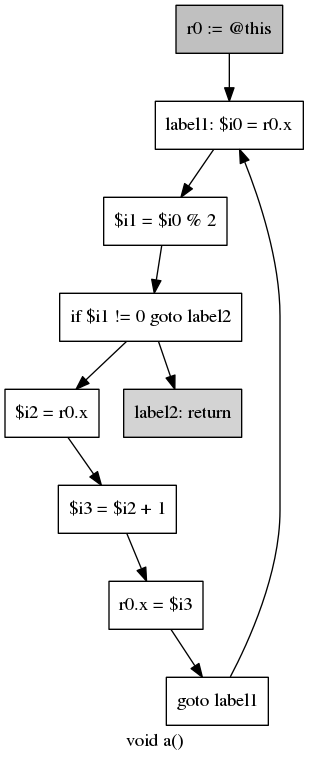
\includegraphics[width=3.5cm, height=6cm]{synchronized.png}
			  \end{figure}
 	\end{columns}
\end{frame}


\begin{frame}[fragile]
  \frametitle{Алгоритм решения задачи. Анализ возможного множества блокировок}
\begin{itemize}
    \item Данная часть алгоритма нужна для предотвращения ложных срабатываний.
    \item Не все локальные переменные могут являться блокировкой.
    \item Если переменная была инициализирована как phi-node, или как не final поле, то она не может являться блокировкой, так как статическим анализом мы не можем узнать ее значение. 
  \end{itemize}
\end{frame}



\begin{frame}[fragile]
  \frametitle{Алгоритм решения задачи. Обход графа}
\begin{itemize}

	\item Для каждой вершины CFG будем хранить множество блокировок($v.locks$), с которыми мы посещали данную вершину.

	\item Также для каждого поля/метода будем сохранять множество блокировок($o.locks$), с которыми к нему обращались.
	\item При обращении к полю $o$ будем пересекать $o.locks$ и взятые в текущий момент блокировки($curLocks$).
	\item Если $o.locks$ стало пустым - значит $o$ не синхронизировано.
\end{itemize}
\end{frame}


\begin{frame}[fragile]
  \frametitle{Алгоритм решения задачи. Обход графа}
\begin{itemize}
	\item При переходе по CFG будем $v.locks$ и $curlocks$. Если $v.locks$ принадлежит $curLocks$, то данную ветвь анализа можно прерывать. Иначе пересекаем $curLocks$ и $v.locks$
	\item При встрече операций синхронизации обновлем $curLocks$.
\end{itemize}
\end{frame}

\begin{frame}[fragile]
  \frametitle{Апробация}
\begin{itemize}
	\item Доступны два режима работы программы: 
	\begin{itemize}
	\item Локальный - Анализирует только приватные поля. Нужен для анализа библиотек. Запускался на билиотеке tomcat. Анализ выделил около 5\% полей.
	
	\item Глобальный - Анализирует любые поля. Нужен для анализа готовых приложений. Запускался на различных клиент-серверных приложениях. Анализ выделил в среднем 7\% полей.
	\end{itemize}
	\item Также в утилиту jDRD, был включен сбор статистики по частоте обращения к найденным полям. Процент обращения к корректно-синхронизированным полям совпадает с процентом найденных полей, что подтверждает полезность работы.
\end{itemize}
\end{frame}

\begin{frame}[fragile]

  \frametitle{Полученные результаты}
  \vspace{0.5cm}
\begin{itemize}
	\setlength\itemsep{1cm}
	\item Разработана утилита, статически определяющая корректно-синхронизированные участки кода.
	\item Утилита была запущена на больших приложениях, показала свою полезность.
	\item Интегрирована c jDRD.
\end{itemize}
\end{frame}

\end{document}
